\section{背景}
  \frame
  {
    \frametitle{\secname~ }
    \begin{block}{凸包围体技术}
      在计算机图形学领域里的各种算法中发挥着重要作用,
      如优化渲染和建模过程,加速求交、碰撞检测等算法。
    \end{block}

    \begin{block}{碰撞检测问题}
   计算机图形学、虚拟现实等领域中的研究热点,
   是计算机模拟真实环境中不可或缺的技术,
   在物理仿真及游戏领域里应用十分广泛。
    \end{block}
  }

  \subsection{凸包围体}
  \frame{
  \frametitle{凸包围体的种类}
  \begin{figure}
  \hspace{-2.0em}
    \begin{minipage}{1.06\textwidth}
    \subfloat[\scriptsize AABB]
        {
           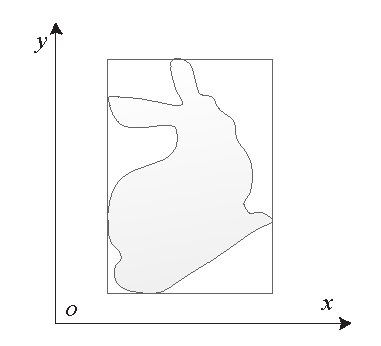
\includegraphics[width=0.2\textwidth]{figures/bunny-2d-AABB.eps}
        }
        \subfloat[\scriptsize OBB]
        {
            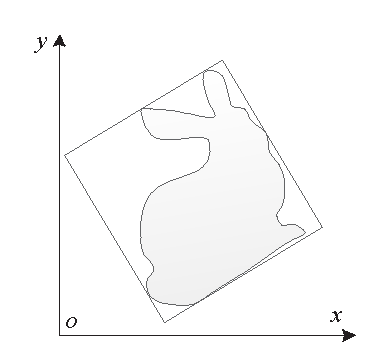
\includegraphics[width=0.2\textwidth]{figures/bunny-2d-OBB.eps}
        }
       \subfloat[\scriptsize Sphere]
        {
           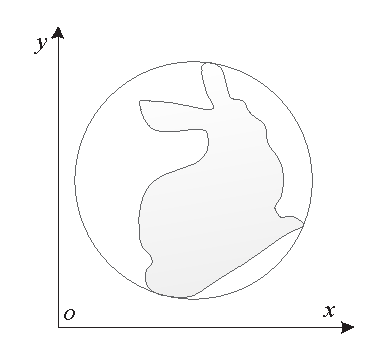
\includegraphics[width=0.2\textwidth]{figures/bunny-2d-Sphere.eps}
        }%\linebreak
        \subfloat[\scriptsize $k$-DOP]
        {
           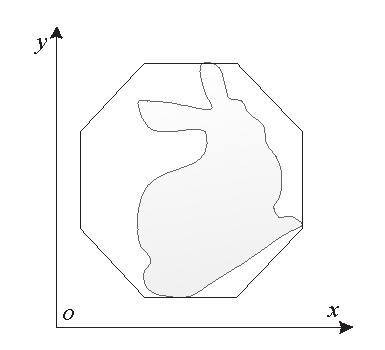
\includegraphics[width=0.2\textwidth]{figures/bunny-2d-8DOP.eps}
        }
        \subfloat[\scriptsize 凸包]
        {
           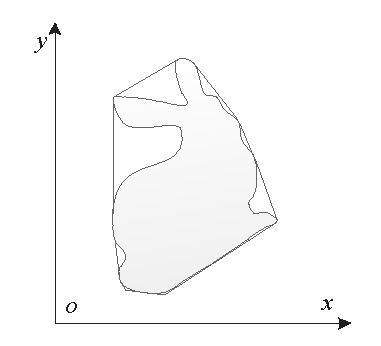
\includegraphics[width=0.2\textwidth]{figures/bunny-2d-Convexhull.eps}
        }
        \end{minipage}
        \caption{不同种类的包围体}
        \label{chart:exps:tightness}
        \end{figure}
        \vspace{-1em}
      其他:Tribox、Swept-sphere、 Sphere-shell、Zonotopes、圆柱形、圆锥、椭球形等等。
  }

      \frame{
   \frametitle{本文目标}
   \begin{block}{综合比较}
     \footnotesize
   \begin{description}
     \item[$k$-DOP\footfullcite{klosowski1998efficient}:]方向固定且有限,不同模型其截面方向一致, 不够紧致。
     \item[凸包:]很(最)紧致, 但面片数量太多, 复杂度$O(n\log n)$。
    \end{description}
  \end{block}
  \begin{block}{本文凸包围体的目标}
     \footnotesize
     \begin{description}
     \item[紧致:] 能够自适应模型,根据模型形状特点有不同的方向;
     \item[快速:] 生成凸包围体的速度要快,利用~GPU~加速;
     \item[灵活:] 通过参数~$k$~调节凸包围体的简单性和紧致程度。
     \end{description}
   \end{block}
  }

  \subsection{碰撞检测算法}
   \frame{
   \frametitle{\subsecname~ }
    
   \begin{block}{碰撞检测算法}
     许多应用的基础,例如在~3D~游戏,物理仿真,机器人,虚拟现实等领域中\footfullcite{ericson2005real}。
   \end{block}

   \begin{block}{分类}
     \begin{description}
       \item[加速结构:] SPT(如四叉树、KD~树等)~v.s~\textbf{BVH}(OBB树、$k$-DOP树等)
       \item[表现形式:] \textbf{刚体}~v.s~可变形,凸体~v.s~凹体,CSG~v.s~参数曲面~v.s~\textbf{多边形网格}
       \item[碰撞环境:] \textbf{成对}~v.s~\textbf{多体},\textbf{静止}~v.s~\textbf{运动},\textbf{离散}~v.s~连续
     \end{description}
   \end{block}
  }

  \frame{
    \frametitle{基于~BVH~的碰撞检测算法}
    \begin{columns}[onlytextwidth]
      \begin{column}{0.35\textwidth}
        \vspace{-1.5em}
        \begin{figure}[htbp]
            \begin{center}
            \begin{boxedminipage}{1\textwidth}
            \subfloat{\label{lbl:bvh-bunny-center-0.png}}
              {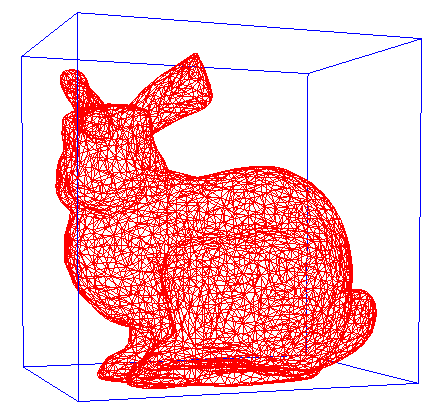
\includegraphics[height=1.4cm]{bvh-bunny-center-0.png}}
            \subfloat{\label{lbl:bvh-bunny-center-1.png}}
              {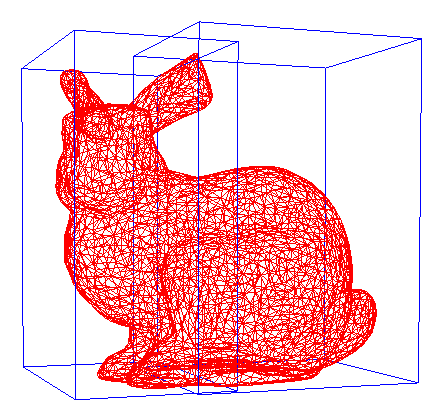
\includegraphics[height=1.4cm]{bvh-bunny-center-1.png}}
            \\
            \subfloat{\label{lbl:bvh-bunny-center-2.png}}
              {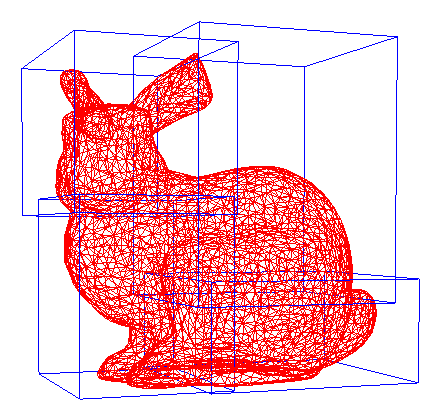
\includegraphics[height=1.4cm]{bvh-bunny-center-2.png}}
            \subfloat{\label{lbl:bvh-bunny-center-3.png}}
              {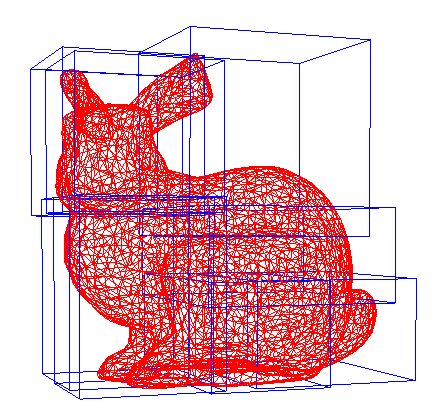
\includegraphics[height=1.4cm]{bvh-bunny-center-3.png}}
            \\\hspace{0.5cm}
            \subfloat{\label{lbl:bvh-bunny-center-4.png}}
              {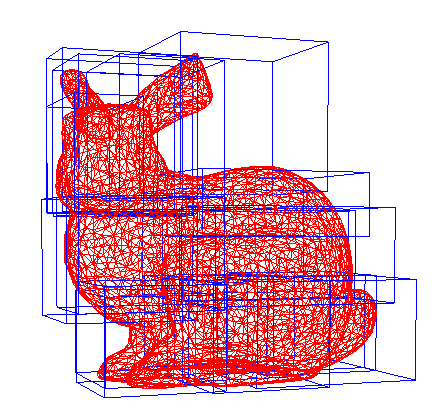
\includegraphics[height=1.5cm]{bvh-bunny-center-4.png}}
            \subfloat{\label{lbl:bvh-bunny-center-5.png}}
              {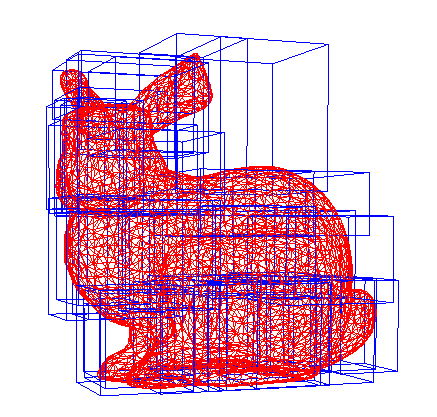
\includegraphics[height=1.5cm]{bvh-bunny-center-5.png}}
            \\
            \subfloat{\label{lbl:bvh-bunny-center-6.png}}
              {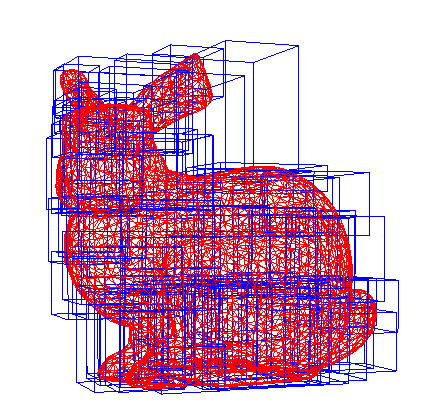
\includegraphics[height=1.5cm]{bvh-bunny-center-6.png}}
            \subfloat{\label{lbl:bvh-bunny-center-7.png}}
              {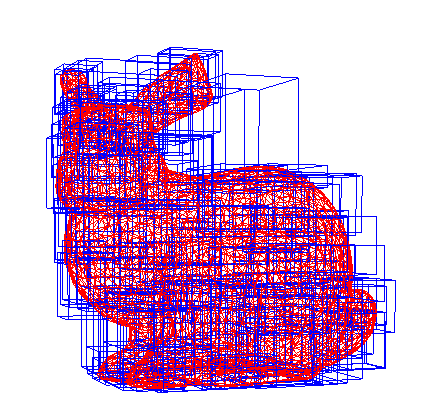
\includegraphics[height=1.5cm]{bvh-bunny-center-7.png}}
            \end{boxedminipage}
            \vspace{-0.5em}
          \caption{八层~BVH~示例}
          \label{lbl:bvh-example}
          \end{center}
          \end{figure}
      \end{column}
      \hspace{0.5em}
      \begin{column}{1.2\textwidth}
      \vspace{0.2em}
         \scalebox{0.5}{
              \begin{minipage}{1.0\textwidth}
      \vspace{-2em}
           \begin{algorithm}[H]
              \caption{自顶向下层次遍历~BVH~}
              \label{alg:traverse-bvh-tree}
              \begin{algorithmic}[1]
              \Require
              两个~BVH~树的根节点~$node_1$,$node_2$
              \Ensure
              模型是否相交
              \Function {TraverseBVHTree}{$node_1, node_2$}
                \If{$node_1.bv \cap node_2.bv = \emptyset$}
                  \State \Return{\textbf{False}}
                  \Comment{包围体重合测试, 包围体不相交直接返回}
                \Else
                    \If {$node_1.children = \emptyset$}
                         \If {$node_2.children = \emptyset$}
                         \State \Comment{最底层叶子节点原生几何相交测试}
                         \State \Return {\Call{CheckIntersection}{$node_1.primitives, node_2.primitives$}}
                         \Else
                            \ForAll {$child \in node_2.children$}
                            \State \Call{TraverseBVHTree}{$node_1, child$} \Comment{递归调用}
                            \EndFor
                         \EndIf
                    \Else
                         \ForAll {$child \in node_1.children$}
                         \State \Call{TraverseBVHTree}{$child, node_2$}  \Comment{递归调用}
                         \EndFor
                    \EndIf
                \EndIf
              \EndFunction
              \end{algorithmic}
              \end{algorithm}
              \end{minipage}
            }
      \\
      %\begin{block}{代价函数}
      \scriptsize \hspace{1em}代价函数: $T_{cost} = n_v * C_v + n_p * C_p + (n_u * C_u)$(运动)
      %\end{block}
      \end{column}
    \end{columns}
}
